\begin{enumerate}
    
    \item If $\sin \theta=0$, then the value of $\tan^2\theta+\cot^2\theta$ is
    \begin{enumerate}
        \hfill\brak{10, 2022}\item $2$
        \hfill\brak{10, 2022}\item $4$
        \hfill\brak{10, 2022}\item $1$
        \hfill\brak{10, 2022}\item $\frac{10}{9}$
    \end{enumerate}
    \hfill\brak{10, 2022}\item $5\tan^2 \theta - 5\sec^2\theta = \underline{\hspace{2cm}}$
    \hfill\brak{10, 2022}\item In  \figref{fig:as.jpeg}, a tower stands vertically on the ground. From a point on the ground, which is $80m$ away from the foot of the tower, the angle of elevation of the tower is found to be $30\degree$. Find the height of the tower.
    \begin{figure}[H]
        \centering
        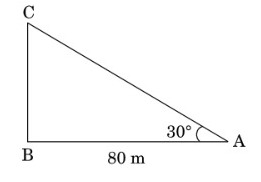
\includegraphics[width=70mm]{cbse-math/figs/as.jpeg}
        \caption{as.jpeg}
        \label{fig:as.jpeg}
    \end{figure}
    \hfill\brak{10, 2022}\item Show that 
    \begin{align}
        \cos(38\degree) \cos(52\degree) - \sin(38\degree)\sin(52\degree) = \cos(90\degree).
    \end{align}
    \hfill\brak{10, 2022}\item Prove that 
    \begin{align}
        \frac{\sin\theta}{\cot\theta+\csc\theta} = 2+\frac{\sin\theta}{\cot\theta-\csc\theta}.
    \end{align}
    \hfill\brak{10, 2022}\item Given 
    \begin{align}
        15 \cot (A) = 8,
    \end{align}
    find the values of $\sin (A)$ and $\sec (A)$.
    \hfill\brak{10, 2022}\item The angles of depression of the top and bottom of a tower as seen from the top of a $60\sqrt{3}m$ high cliff are $45\degree$ and $60\degree$ respectively. Find the height of the tower. (Use $\sqrt{3}=1.73$)
    \hfill\brak{10, 2022}\item The angle of elevation of the top of a building from the foot of the tower is $30\degree$ and the angle of elevation of the top of the tower from the foot of the building is $60\degree$. If the tower is $50$ meters high, then find the height of the building.
    \hfill\brak{10, 2022}\item From a point on a bridge across a river, the angles of depression of the banks on opposite sides of the river are $30\degree$ and $60\degree$ respectively. If the bridge is at a height of $3$ meters from the banks, then find the width of the river. 
    \hfill\brak{10, 2022}\item In \figref{fig:ak}, Gadisar Lake is located in the Jaisalmer district of Rajasthan. It was built by the King of Jaisalmer and rebuilt by Gadsi Singh in the $14$th century. The lake has many Chhatris. One of them is shown below:
    \begin{figure}[H]
        \centering
    	 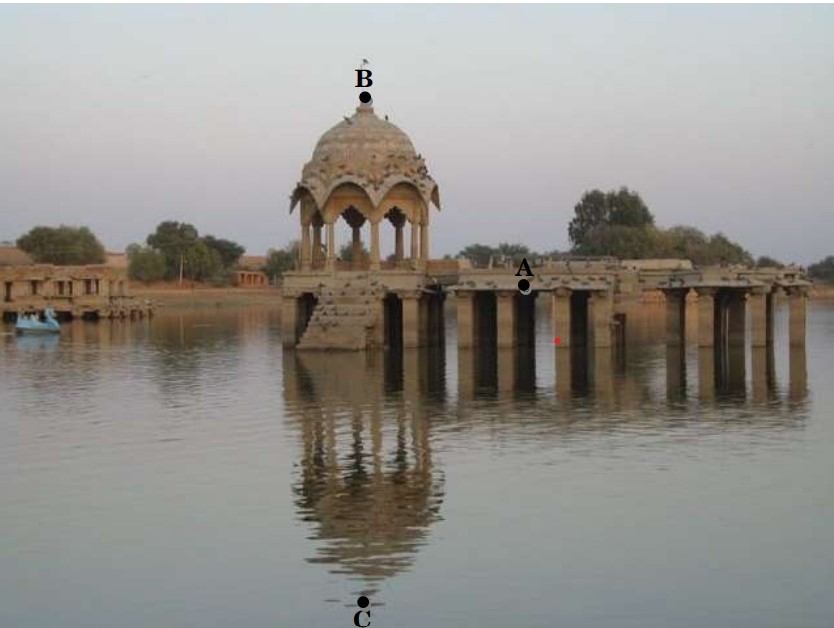
\includegraphics[width=70mm]{cbse-math/figs/ak.jpeg}
        \caption{ak.jpg}
        \label{fig:ak}
    \end{figure}
    Observe the picture. From a point $A$ $h$ meters above the water level, the angle of elevation of the top of Chhatri (point $B$) is $45\degree$ and the angle of depression of its reflection in the water (point $C$) is $60\degree$ . If the height of Chhatri above water level is (approximately) $10$ meters, then 
    \begin{enumerate}
        \hfill\brak{10, 2022}\item Draw a well-labeled figure based on the above information.
        \hfill\brak{10, 2022}\item Find the height ($h$) of the point $A$ above water level. (Use $\sqrt{3}=1.73$) 
    \end{enumerate}

    \hfill\brak{10, 2022}\item In \figref{fig:su.jpeg}, from a point on a bridge across a river, the angles of depression of the banks on opposite sides of the river are $30\degree$ and $45\degree$. If the bridge is at a height of $8$ meters from the banks, then find the width of the river.
    \begin{figure}[H]
        \centering
        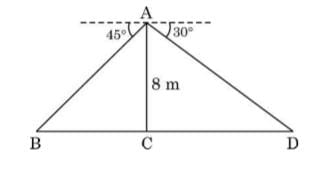
\includegraphics[width=70mm]{cbse-math/figs/su.jpeg}
        \caption{su.jpg}
        \label{fig:su.jpeg}
    \end{figure}
    
    \hfill\brak{10, 2022}\item Case Study-1:
    
    In \figref{fig:kite.jpeg}, Kite Festival is celebrated in many countries at different times of the year. In India, every year on $14^{th}$ January is celebrated as International Kite Day. On this day, many people visit India and participate in the festival by flying various kinds of kites.
    
    \begin{figure}[H]
	\centering
        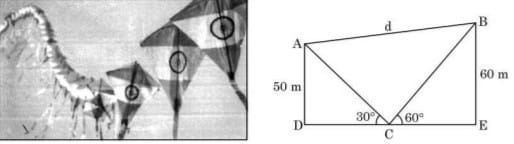
\includegraphics[width=70mm]{cbse-math/figs/kite.jpeg}
        \caption{kites}
        \label{fig:kite.jpeg}
    \end{figure}
    
    In Fig. 5, the angles of elevation of two kites (Point $A$ and $B$) from the hands of a man (Point $C$) are found to be $30\degree$ and $60\degree$ respectively. Taking $AD = 50$ meters and $BE = 60$ meters, find:
    \begin{enumerate}
        \hfill\brak{10, 2022}\item The lengths of strings used (take them straight) for kites $A$ and $B$ as shown in the figure.
        \hfill\brak{10, 2022}\item The distance $d$ between these two kites.
    \end{enumerate}
    
    
    \hfill\brak{10, 2022}\item Two boats are sailing in the sea $80$ meters apart from each other towards a cliff $AB$. The angles of depression of the boats from the top of the cliff are $30\degree$ and $45\degree$ respectively, as shown in \figref{fig:boat.jpeg}
    
    \begin{figure}[H]
        \centering
        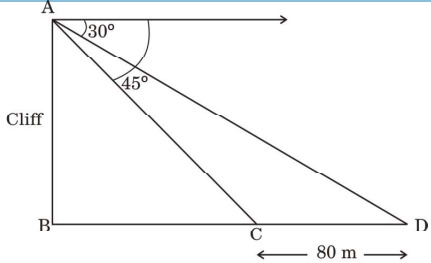
\includegraphics[width=70mm]{cbse-math/figs/boat.edit.jpeg}
        \caption{boat}
        \label{fig:boat.jpeg}
    \end{figure}
    
    Find the height of the cliff.
    
    \hfill\brak{10, 2022}\item The angle of elevation of the top $Q$ of a vertical tower $PQ$ from a point $X$ on the ground is $60\degree$. From a point $Y$, $40$ meters vertically above $X$, the angle of elevation of the top $Q$ of tower $PQ$ is $45\degree$. Find the height of the tower $PQ$ and the distance $PX$. (Use $\sqrt{3} = 1.73$)
    
    \hfill\brak{10, 2022}\item An Aeroplane at an altitude of $200$ meters observes the angles of depression of opposite points on the two banks of a river to be $45\degree$ and $60\degree$. Find the width of the river. (Use $\sqrt{3} = 1.732$)
    
    \hfill\brak{10, 2022}\item From the top of an $8$ meter high building, the angle of elevation of the top of a cable tower is $60\degree$ and the angle of depression of its foot is $45\degree$. Determine the height of the tower. (Take $\sqrt{3} = 1.732$).
    
    \hfill\brak{10, 2022}\item As observed from the top of a lighthouse $60$ meters high from the sea level, the angles of depression of two ships are $45\degree$ and $60\degree$. If one ship is exactly behind the other on the same side of the lighthouse, then find the distance between the two ships. (Use $\sqrt{3} = 1.732$)
    
    \hfill\brak{10, 2022}\item At a point on the level ground, the angle of elevation of the top of a vertical tower is found to be $\alpha$, such that $\tan\alpha = \frac{5}{12}$. On walking $192$ meters towards the tower, the angle of elevation $\beta$ is such that $\tan\beta = \frac{3}{4}$. Find the height of the tower.
    
    \hfill\brak{10, 2022}\item $\tan^{-1}\frac{1}{\sqrt{3}} - \cot^{-1}\frac{-1}{\sqrt{3}}$
    
    \hfill\brak{10, 2022}\item Two angles of a triangle are $\cot^{-1}2$ and $\cot^{-1}3$. The third angle of the triangle is?
    
    \hfill\brak{10, 2022}\item Solve for $x$:
    \begin{align}
        \sin^{-1}(1-x) - 2 \sin^{-1} x = \frac{\pi}{2}
    \end{align}
\hfill\brak{10, 2022}
\end{enumerate}
